\chapter{Detector}\label{c:Det}

\section{The Large Hadron Collider}

	The Large Hadron Collider (LHC) is a circular particle accelerator operated at European Organisation for Nuclear Research (CERN, Conseil Europ\'{e}en pour la Recherche nucle\'{e}aire). Currently the largest accelerator in the world, the LHC is designed to collide heavy ions or opposing proton beams for a peak design centre-of-mass energy $\sqrt{s}=14$TeV with a luminosity of $10^{34}$cm$^{-2}$s$^{-1}$ \cite{lhc}. The forst proton beams were circulated in the LHC in 2008, with Run 1 of LHC data taking being conducted until 2013, at which point the machine was shut down for maintenance. Following on from the initial operations, Run-2 of the LHC has been undergoing since 2015, operating at $\sqrt{s}=13$TeV. \todo{need to explain the concept of luminosity somewhere?}

	The principle LHC ring consists of eight pairs of alternating long arc sections and short straight insertion sections, situated within the underground tunnel excavated for the older Large Electron Positron Collider experiment \cite{lep1, lep2}. The arc sections contain the dipole magnets used to bend the particle beam around the ring, while the straight sections contain four interaction points, at each of which the large experiments are located. The remaining straight sections contain the operational systems of the LHC: beam acceleration, injection,  dumping and collimation. The proton beams are genereated outside the principle ring and inserted into the ring by the LHC injector chain, a syequence of smaller accelerators which are used to bring the proton beams up to a suitable energy for injection. The proton beams are arranged such that the protons move in bunches of $\mathcal{O}(10^{11})$ protons, with multiple byunches placed into trains. Once a beam is accelerated to the target energy interactions begin, at which point a steady stream of interactions is produced until the beam is replaced due to general decay of the interaction fate or beam instabilities.

	The large experiments at the LHC are ATLAS (A Toroidal LHC ApparatuS), CMS (Compact Muon Solenoid), LHCb (LHC beauty) and ALICE (A Large Ion Collider Experiment). LHCb is a forward spectrometer heavy flavour experiment, designed to study flavour physics with emphasis on the $b$ quark and on matter/anti-matter asymmetry. ALICE focuses on the collisions of heavy ions, while ATLAS and CMS are general purpose detectors to conduct experiments across a broad range of modern physics research areas.

	\subsection{Run Conditions in 2016}

	Over the course of 2016 the LHC beam was operated predominantly with two beams of energy 6.5TeV for $\sqrt{s}=13$TeV following beam commissioning runs. Over the course of the 2016 data-taking the ATLAS and CMS experiments achieved an integrated luminosity of $40$ fb$^{-1}$ with a peak instantaneous luminosity of $1.4\times10^{34}$cm$^{-2}$s$^{-1}$ with 2220 bunches per beam \cite{Run2016}. \todo{Definitely think something to do with lumi might be needed somewhere, and on byunchspacings}


\section{The ATLAS Detector} \todo{Detail level?}

	The ATLAS detector \cite{ATLAS} is a multi-detector designed to manage with the experimental conditions of the LHC and study a broad selection of physics phenomena. The detector is cylindrical in structure with the axis alignewd to the beam path and nominally forward-backward symmetric in terms of the beam collision point at the centre of the detector. The detector provides approximately $4\pi$ solid angle coverage around the interaction point to detect as many collision products as possible.

	The structure of the ATLAS detector is composed of concentric subsystems around the interaction point.  The Inner Detector is the component closest to the interaction point, and is contained in a superconducting solenoid. This is surrounded by high-granularity calorimeters and an extensive muon spectrometer contained within and eight-fold azimuthally symmetric arrangement of three large toroidal magnets. A schematic representation of the ATLAS detector is shown in Figure \ref{fig:t:ATLAS}. 	The subsystems are arranged into three cryostats, two \textit{endcaps} located on the ends of the detector and the central \textit{barrel} section. Discussion of the coordinates and quantities used in the detector is found in Section \ref{t:geometry}. A summary of the operational paramaters of the principle detector components is given in Table \ref{tab:t:operational}.

	\begin{figure}[h]
		\centering
		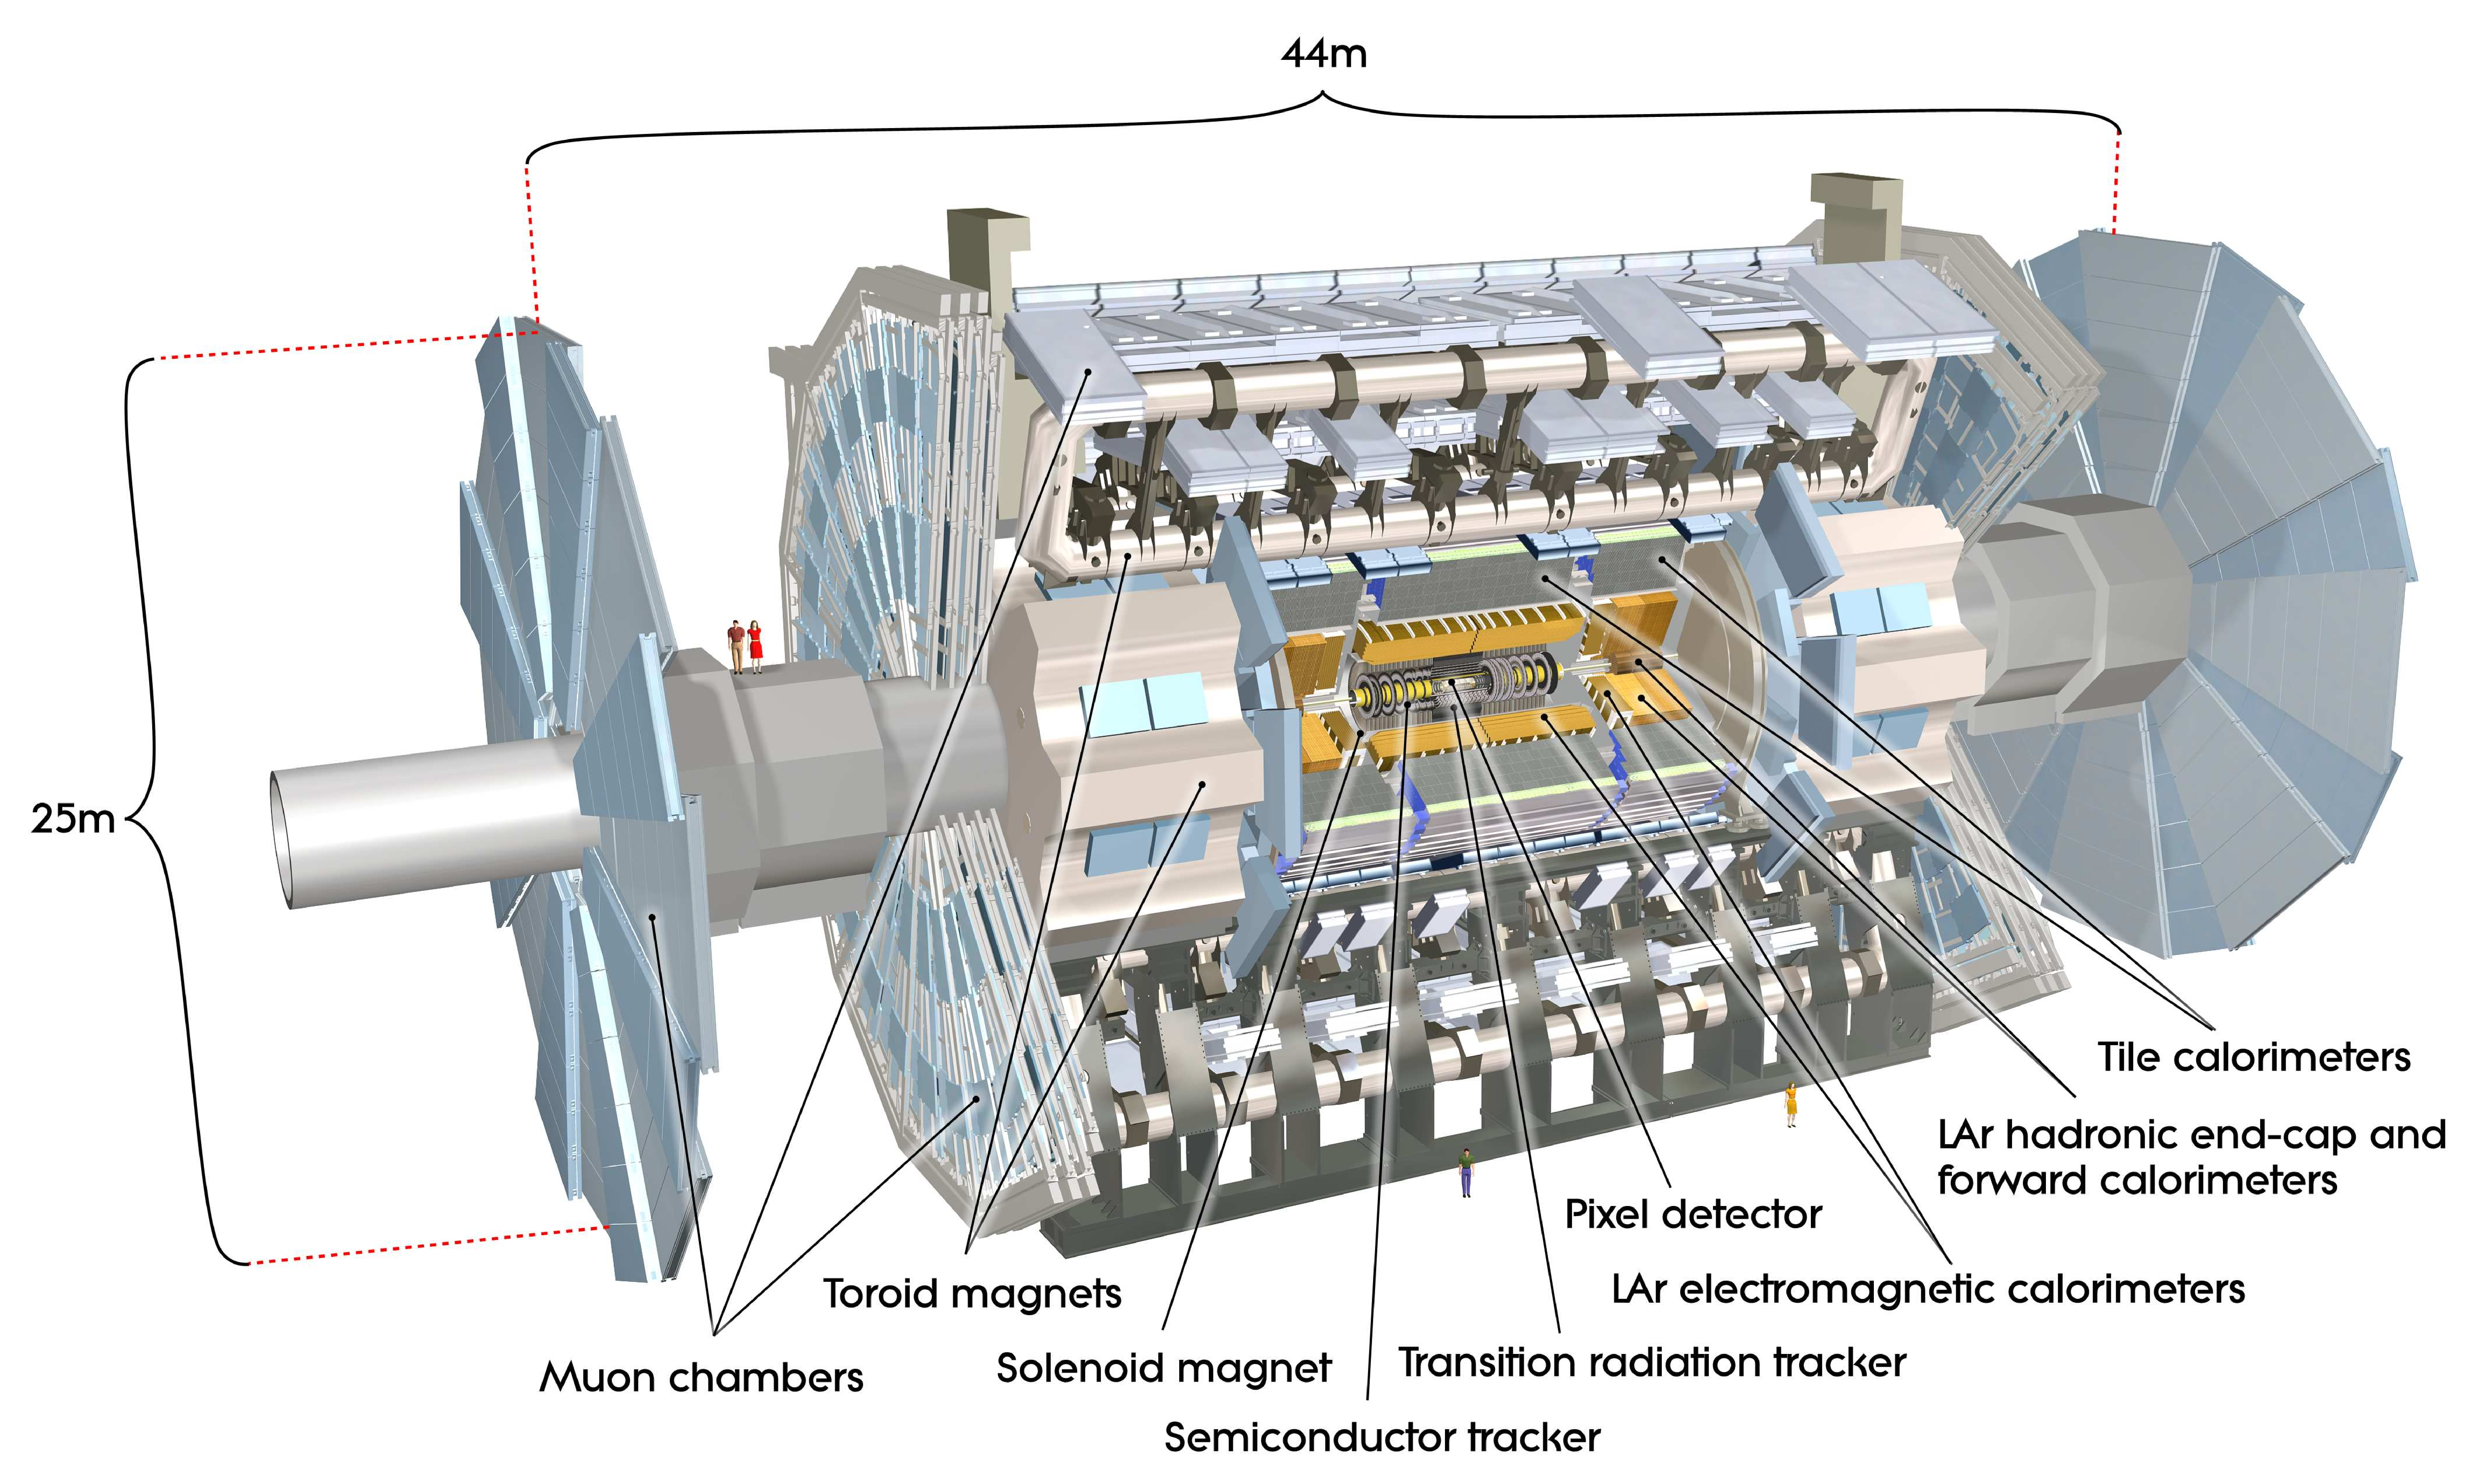
\includegraphics[width=0.7\linewidth]{D/FIGS/ATLAS_SE_Corrected7}
		\caption{Schematic cut-away of the ATLAS detector \cite{ATLASSchem}.}
		\label{fig:t:ATLAS}
	\end{figure}



	\subsection{Inner Detector}

		The Inner Detector (ID) provides pattern recognition, momentum measurements, electron identification and measurements of both primary and secondary vertices to efficiently identify jets containing \bhadron within a pseudorapidity range $|\eta|<2.5$. The ID itself is contained within a 2 T solenoidal field, and makes use of a combination of slilicon pixel and strip detectors at the core of the tracking volume wrapped with straw-tube tracking detectors in the Transition Radiation Tracker to perform particle identification and tracking.

	\subsection{Calorimeters}

		Calorimeters are used to measure the energy of any particle incident into the calorimeter. Incident particles cause the development of either Electromagnetic (EM) or hadronic showers within the calorimeter substrate, and the energy deposited in this shower can be used to calculate the incident energy. The ATLAS calorimetry system consists of a combination of EM and hadronic calorimeters arranged with full $\phi$-symmetry around the beam axis. The combination of all separate calorimeters provides pseudorapidity coverage in the range $|\eta| < 4.9$. Within the pseudorapidity region of the inner detector, the fine granularity of EM calorimeters is optimised for measurements of electron and photon tracks and momenta, while the coarser hadronic calorimeters contained in the remainder of the calorimeter system are sufficient for jet reconstruction and missing energy calculations. The structure and design of the calorimeter components has been optimised to provide complete azimuthal coverage, take into account the engineering requirements for assembling the detector for desired calorimitry performance and account for radiation considerations between the different detector components \cite{ATLAS}.

		The EM calorimeter is a lead-Liquid-Argon (LAr) detector, which is split into a barrel section (EMB, $|\eta|<1.475$) and two endcap sections (EMEC, $1.375<|\eta|<3.2$) with each section contained in a separate cryostat. The EMB consists of two identical half-barrels split by a small gap at $z=0$. Each of the EMEC sections is a pair of coaxial wheels, with the inner and outer sections covering regions $1.375<|\eta|<2.5$ and $2.5<|\eta|<3.2$ respectively.

		Hadronic calorimetry for particles undergoing the strong interaction is provided by the steel/scintillator tile calorimeter for pseudorapidity values of $|\eta|<1.7$, and by the LAr flat-plate Hadronic Endcap Calorimeter (HEC) for $1.5<|\eta|<3.2$. The tile calorimter directly surrounds teh EM calorimeter, and is split into a central barrel section for $|\eta| < 1.0$ and two extended barrel sections covering $0.8<|\eta|<1.7$. The HEC akin to the EMEC consists of two separate wheels per end-cap covering $1.5<|\eta|<3.2$, and is contained within the same cryostat as the EMEC. The detector consists of alternating copper plates with LAr gaps to act as the active medium.

		In addition to the barrel and end-cap calorimeters, the LAr Forward Calorimeter is contained within the end-cap cryostat (The FCal is omitted from Figure \ref{fig:t:ATLAS}) and is designed to perform both EM and hadronic calorimetry across a pseudorapidity range of $3.1<|\eta|<4.9$ using a combination of copper/LAr (EM) and tungsten/LAr (hadronic) calorimeter components.

	\subsection{Muon Spectrometer}

		The muon spectrometer is the outermost component of the ATLAS detector, measuring trajectory and momentum of muons from the interactions within a pseudorapidity range of $|\eta| < 2.7$. The muon system consists of three large superconducting coils that deflect the muon trajectories. The system is designed for high precision tracking of the minimally ionising muons and for use in the triggering system.


	  	\begin{table}[ht]
	  		\caption{Performance goals and operational ranges for principle components of the ATLAS detector. \cite{ATLAS}}
	  		\label{t:tab:operational}
	  		\medskip
	  		\centering
	  		\begin{tabular}{llll}\toprule
	  			System & Component & $\eta$ Coverage & Resolution \\\midrule
	  			Tracking &  & $0<|\eta|<2.5$ & $\sigma_{p_\text{T}}/p_\text{T} = 0.05\% p_\text{T}\oplus1\%$\\
	  			EM Calorimetry & EMB & $0<|\eta|<1.475$ & $\sigma_{E}/E = 10\%/\sqrt{E} \oplus0.7\%$ \\
	  			& EMEC (Inner) & $1.375<|\eta|<2.5$ &  \\
	  			& EMEC (Outer) & $2.5<|\eta|<3.2$ &  \\
	  			Hadronic Calorimetry & Tile (Barrel) & $0<|\eta|<1$ & $\sigma_{E}/E = 50\%/\sqrt{E} \oplus3\%$ \\
	  			& Tile (Extended) & $0.8<|\eta|<1.7$ &  \\
	  			 & HEC & $1.5<|\eta|<3.2$ &  \\
	  			Forward Calorimetry & FCal & $3.1<|\eta|<4.9$ & $\sigma_{E}/E = 100\%/\sqrt{E} \oplus10\%$ \\
	  			Muon Spectrometer &  &  $0<|\eta|<2.7$  & $\sigma_{p_\text{T}}/p_\text{T} = 10\%\,at\,p_\text{T}=1$ TeV  \\\bottomrule
	  		\end{tabular}\\[5pt]
	  	\end{table}
	  	\todo{remember what this is}

\section{Triggers}

	When operating at the design luminosity, the LHC produces a bunch-crossing rate of 40 MHz \cite{trigrun22017}. This extreme rate of interaction necessitates a trigger system to reduce the output rate to a suitable level for offline processing, which is predominantly limited by the rate at which data can be written to disk. The limit of the output rate is determined by the computational capabilities, specifically the average data rate of output. The trigger system selects events by quickly identifying distinguishing features of events (i.e. signatures of muons, electrons, jet and \bjet objects) and using combinations of these signatures to signify an event as relevant for further analysis. Overall usage of the trigger system brings the output rate down to 1 kHz with a maximum L1 rate of 100 kHz.

	The ATLAS trigger system consists of a chain of selection stages of increasing severity and corresponding decrease in rate. A schematic outline of the trigger system is shown in Figure \ref{fig:d:trigger}. This outline covers both the logical process and the transfer of data between components of the trigger chain. The principle decision logic of the trigger system is however contained in two sections, the L1 trigger sytem and the High Level Trigger (HLT).

	\begin{figure}
		\centering
		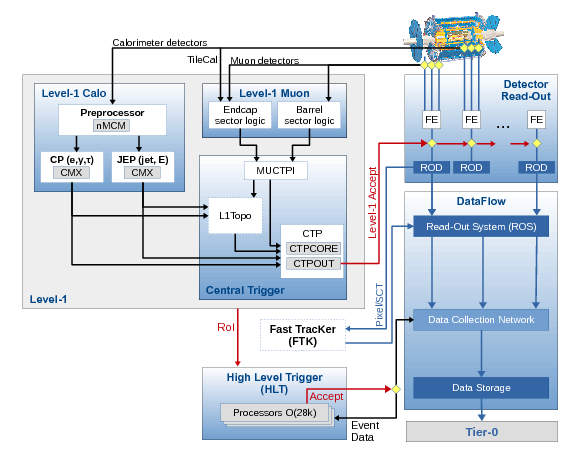
\includegraphics[width=0.7\linewidth]{D/FIGS/trigschem}
		\caption{Schematic plot of the ATLAS Trigger and Data acquisition system \cite{trig2015}.}
		\label{fig:trigschem}
		\end{figure}\todo{THis is not a suitable plot}

	The L1 trigger system \cite{L1} is a hardware based decision system, using fast custom electronics to minimise latency in any decision. The L! uses reduced-granularity data from the calorimetric and muon detectors, reconstructed objects and missing and total transverse energy. The high bunch-crossing rate means instantaneous\note{word choice} processing of the event is non-viable, so event readouts are stored in a buffer chain of events to be evaluated with a fixed permitted decision time per event. Along with this first selection, the L1 trigger defines \textit{Regions of Interest} (RoIs) in the phase space within the detector, which are labelled for investigation in the HLT. TALK ABOUT RATE

	In contrast to the hardware computation of the L1 system, the HLT consists of software algorithms running in a farm  of $\approx40000$ interconnected processors\cite{trigrun22017}. Following acceptance of an event by the L1 trigger, events are transferred from the initial data pipeline to dedecated readout buffers for the HLT. The HLT performs processing on the events using finer-granularity information from teh calorimeters and muon spectrometer, along with making use of information from the ID, which is unavailable to L1. This more precise data is the computed using object reconstruction algorithms similar to the offline reconstruction. A decision at HLT level is managed by a trigger chain, which is a sequence of specific criteria and algorithms evaluated on an event in sequence. The HLT provides $\mathcal{O}(1000)$ independent trigger chains for evalutating events. Along with the partial reconstruction of relevant objects, the HLT is capable of performing complete reconstruction of an event, and also capable of writing out these partial or complete reconstructions of an event into different data streams from the complete detector readout for use in analysis.


\section{Object Reconstruction}

	\subsection{Jets}

	As discussed in Section \ref{t:hadronisation} the coloured fragments produced during collisions produce collimated streams of hadrons called jets, which are the physical objects detected in the event. Detectors make use of algorithms to reconstruct these jets from the calorimiter readouts to relate the stream of hadrons to the initial fragmented partons. There are various algorithms used to reconstruct jets within the ATLAS detector, and these algorithms commonly require the definition of a jet to be invariant under additional soft or collinear emissions from the hadron jet. Such algorithms are designated as infra-red (IR) or collinear safe.

	Modern jet algorithms are broadly split into cone-type al

	The principle algorithm used for jet reconstruction at ATLAS is the anti-$k_t$ algorithm \cite{antikt}


	ENERGY SCALES

\section{\textit{b}-Tagging}
\label{det:btagging}

	Identification of \bquark jets in ATLAS is based on combining the output of three separate \btag algorithms: Impact Parameter based (IP2D and IP3D, described in Section \ref{det:btag:ip}), Secondary Vertex based (SV, described in Section \ref{det:btag:sv}) and Decay Chain based (JetFitter, described in Section \ref{det:btag:jf})into a multivariate discriminant (MV2, covered in Section \ref{det:btag:mv}) which is used to distinguish the jet flavours. These algorithms have undergone continuous improvement over the Run-2 cycle of the LHC to improve the separation of jet flavours.

	\subsubsection{IP2D and IP3D: Impact Parameter based Algorithms}
		\label{det:btag:ip}

		The typical topology for a \bhadron of a secondary vertex displaced from the hard scatter interaction point as a results of the lifetime of \bquark is used as the basis of these algorithms. Impact parameters of tracks from the secondary vertex are computed with respect to the primary vertex of the interaction. The IP2D algorithm uses a transverse impact parameter ($d_0$) defined as the distance of closest approach of a track to the  primary vertex in $r$-$\phi$ plane around the vertex. The IP3D algorithm uses both the transverse and a correlated longitudinal impact parameter ($z_0\sin\theta$), defined as the distance between the point of closest approach in $r$-$\phi$ and the primary vertex in the longitudinal plane. \todo{I kind of want a diagram here, but that doesn't appear to be the norm}. These parameters typically have large values as a result of the lifetime of \bquark. The signs of the impact parameters are also defined to take account of if they lie infront or behind the primary vertex with respect to the jet direction, with secondary vertices occuring behind the primary vertex normally due to background.

		The significance of the impact parameter values ($\frac{d_0}{\sigma_{d_0}}$, $\frac{z_0}{\sigma_{z_0\sin\theta}}$) for each track are compared to probability density functions obtained from reference histograms derived from Monte Carlo simulation, with each track being compared to a selection of reference track categories. This results in weights which are combined using a log-likelihood ratio (LLR) discriminant to compute an overall jet weight separating the $b$, $c$, and light-jet flavours from each other. \cite{btagOptimisation, bTagPerformance}

	\subsubsection{SV1: Secondary Vertex Finding algorithm}
	\label{det:btag:sv}

		The secondary vertex algorithm uses the decay products of the \bhadron to reconstruct a distinct secondary vertex. The algorithm uses all tracks that are significantly displaced from the primary vertex associated with the jet, forming vertex candidates for all pairs of track, while rejecting any vertices that would be associated with decay of long lived particles (e.g. $K_s$, $\Lambda$), photon conversions or interactions with the material in the detector. The tracks forming these vertex candidates are then iteratively combined and refined to remove outliers beyond a $\chi^2$ threshold leaving a single inclusive vertex.

		The properties of this secondary vertex are used to differentiate the flavour of the jet. The SV1 algorithm is based on a LLR formalism similar to the IP algorithms, and makes use ot the invariant mass of all charged tracks used to reconstruct the vertex, the number of two track vertices and the ratio of the invariant mass of the charged tracks to the invariant mass off all tracks. In addition the algorithm is signed in a similar fashion to the IP algorithms and uses the $\Delta R$ between the jet direction and secondary vertex displacement direction in the LLR calculation. The algorithm uses distributions of these variables to distinguish be      tween the jet flavours. \cite{btagOptimisation, bTagPerformance} \note{Might be worth mentioning the way these are trained}

	\subsubsection{JetFitter: Decay Chain Multi based Algorithm}
	\label{det:btag:jf}

		The JetFitter algorithm exploits the topological structure of weak \bhadron and \chadron decays inside the jet to reconstruct a full \bhadron decay chain. A Kalman filter \todo{Either understand or just cite} is used to find a common line between the on which lie the $b$, $c$ and primary vertices to approximate the \bhadron flight path. A selection of variables relating to the primary vertex and the properties of the tracks associated with the jet are used as input nodes in a neural network. This neural network uses the input variables and \pt and $|\eta|$ variables from the jets, reweighted in the kinematic variables to ensure the spectra of the kinematics are not used in the training of the neural net. The neural network outputs a discriminating variable relating to each jet flavour which are used to tag the jets. \cite{btagIdentification}

	\subsection{Multivariate Algorithm}
	\label{det:btag:mv}

	The output variables of the three basic algorithms described prior are combined as input into the Multivariate Algorithm MV2. MV2 is a Boosted Decision Tree (BDT) algorithm which has been trained on $t\bar{t}$\note{Why?} events to discriminate \bjets from light and \cjets. The algorithm makes use of the jet kinematics in addition to the tagger input variables to prevent the kinematic spectra of the training sample from being used as discriminating factor. \note{list all input variables?} The MV2 algorithm is an revised version of the MV1 algorithm used during Run-1 of the LHC, and has three sub-variants (MV2c00, MV2c10, and MV2c20) of the algorithm distinguished by the exact background composition of the training sample. The naming convention initially referred to the \cjet composition of the training sample, e.g. for MV2c20 the \bjets are designated as signal jets where a mixture of 80\% light jets and 2-\% \cjets was designated as background.

	The MV2 algorithm has a set of working points, defined by a single value of the output distribution of the algorithm, which are configured to provide a specific \bjet selection efficiency on the training $t\bar{t}$ sample. Rather than being used independently, physics analyses will make use of several working points as an increase in \bjet efficiency (corresponding to \textit{looser} \bjet selection) will bring an increased mistag rate of light and \cjets.

	These algorithms were refined prior to the 2016 Run-2 data-taking session in response to \cjets limiting physics analyses more the light-jets. This change  to enhance the \cjet rejection meant that for the MV2c10, the \cjet fraction was set to 7\% in training and the fraction for MV2c20 was 15\%. There were a selection of other improvements to the algorithm made to the algorithm relating to the BDT training parameters and the use of the basic algorithms before the 2016 data taking. With these refinements, the MV2c10 algorithm was found to provide a comparable level of light-jet rejection to the original 2015 Mv2c20 algorithm with impoved \cjet rejection, so was chosen as the standard \btag algorithm for 2016 analyses. \cite{btagOptimisation}


\section{Trigger Level Analysis}


\endinput
